\chapter{\bf Mas então o que é a realidade virtual?}
\paragraph{}
\section{Formação léxica da palavra.}
\paragraph{}
Podemos facilmente decompor Realidade Virtual em duas simples palavras: "Realidade" e "Virtual".
\begin{enumerate}
\item[\bf{Virtual: }]Virtual é algo "que tem a força de exercer-se, mas que não se exerce", "suscetível a realizar-se";"é algo feito ou simulado através de meios eletrónicos"\cite{7}.
\item[\bf{Realidade: }]Realidade é a existência efetiva de algo;
\end{enumerate}

Podemos então concluir que o termo "Realidade Virtual" significa que é possivel criar ou simular algo que realmente existe mas que apesar de tudo não é verdadeiro.
\section{Conceito}
\paragraph{}
	Toda a realidade que experienciamos, é apenas uma combinação de todos os nossos sentidos(ex:audição,olfato,etc...), e esta tecnologia serve-se desses mesmos sentidos para gerar um ambiente e uma interação não real de maneira a enganar a perceção do utilizador sobre o meio onde se encontra.
	\begin{figure}
	\center
	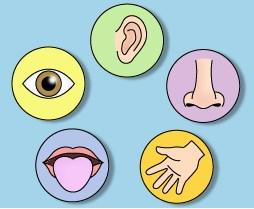
\includegraphics[scale=0.4]{imagens/sentidos.jpg}
	\caption{5 sentidos principais do corpo humano.\cite{1} }
	\end{figure}
	
	A Realidade Virtual é então uma "forma de visualizar,manipular, explorar,interagir e modificar dados complexos através do computador"\cite{8} que interfere com os nossos sentidos de maneira a criar uma sensação de falsa realidade.
	
	"Atualmente esta tecnologia é conseguida através de equipamentos tecnológicos tal como capacetes , monitores e luvas, que servem para ampliar a estimulação dos sentidos" \cite{9}
	"No entanto o nosso cérebro não é fácil de enganar, visto que os nossos sentidos e o nosso cérebro evoluiram de maneira a que todo o nosso redor esteja perfeitamente sincronizada" o que faz com que ao minimo erro nesta tecnologia, nós conseguimos diferenciar o real do imaginário.Nasce então assim a politica dos 3 Is na Realidade Virtual.Para tirarmos proveito desta tecnologia ao máximo,a mesma tem de obedecer a 3 simples passos:
	\begin{enumerate}
	\item[1]- \textbf{Imersão:}Qualquer software e hardware de realidade virtual tem de ser imersivo, servindo-se dos sentidos do ser humano para o fazer.
	\item[2]- \textbf{Interação:} maneira a captar a atenção do nosso cérebro, tem de existir uma interação entre homem-máquina.Cada vez mais são inventados novos géneros de hardware sofisticados que permitam esta interação ser cada vez mais real.
	\item[3]- \textbf{Imaginação:} Um programa que usufrui desta tecnologia tem obrigatoriamente de estimular a imaginação do utilizador.Se isso não acontecer, não é possivel criar a sensação de uma realidade alternativa.
	\end{enumerate}

	
	\begin{figure}
	\center
	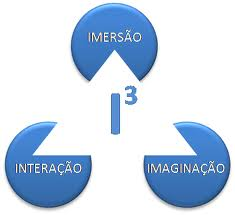
\includegraphics[scale=0.5]{imagens/3is.jpg}
	\caption{Representação da trilogia dos 3 I's \cite{2}}
	\end{figure}
